\section{Managing a bibliography}

\begin{frame}[fragile]{BibTeX}
  \href{https://ctan.org/pkg/bibtex?lang=en}{BibTeX}
  can be used to manage bibliographies.
  (\href{https://ctan.org/pkg/biblatex?lang=en}{BibLaTeX}
  is a more sophisticated alternative.)

  \begin{itemize}
    \item BibTeX entries are stored in a \texttt{.bib} file
    \item I recommend maintaining a \emph{single} centralised \texttt{.bib}
      file for the duration of your PhD.
  \end{itemize}
\end{frame}

\begin{frame}[fragile]{BibTeX entries}
  A list of entry types which BibTeX understands can be
  \href{http://bib-it.sourceforge.net/help/fieldsAndEntryTypes.php#Entries}%
    {found here}.

  \begin{lstlisting}
@book{knuth84,
 title="The texbook",
 author="{Donald Ervin} Knuth and Duane Bibby",
 volume="3",
 year="1984",
 publisher="Addison-Wesley Reading"
}
  \end{lstlisting}
\end{frame}

\begin{frame}[fragile]{Referencing with BibTeX}
  \begin{itemize}
    \item References are included as \lstinline|\cite{knuth84}|, where
      \texttt{knuth84} is the \lstinline|title| of a BibTeX entry
    \item Include your \texttt{.bib} file with
      \lstinline|\bibliography{references}|, where \texttt{references} is the
      name of your file
  \end{itemize}
\end{frame}

\begin{frame}[fragile]{\text{\href{https://ctan.org/pkg/natbib?lang=en}%
                                  {\color{white} \tb usepackage\{natbib\}}}}
  \begin{itemize}
    \item \href{https://ctan.org/pkg/natbib?lang=en}{natbib} can be used to
      implement author-year citations.
    \item Introduces commands \lstinline|\citep| and \lstinline|\citet|, to
      cite in parenthesis or text.
    \item \lstinline|\citep*| and \lstinline|\citet*| print full author list
    \item Multiple citations can be made as \lstinline|\citep{paper1, paper2}|
  \end{itemize}
\end{frame}

\begin{frame}{Compiling with BibTeX}
  BibTeX adds extra complexity to the processing of your manuscript. You will
  have to run \LaTeX\ a number of times.

  \alert{1.} pdflatex thesis.tex

  \alert{2.} bibtex thesis.\alert{aux}

  \alert{3.} pdflatex thesis.tex

  \alert{4.} pdflatex thesis.tex

  A Makefile can simplify compilation. However, I'd recommend using
  \href{https://ctan.org/pkg/latexmk?lang=en}{latexmk}.
\end{frame}

\begin{frame}{Citations from Google Scholar}
  Google scholar can be used to export citations easily.
  \begin{figure}
    \centering
    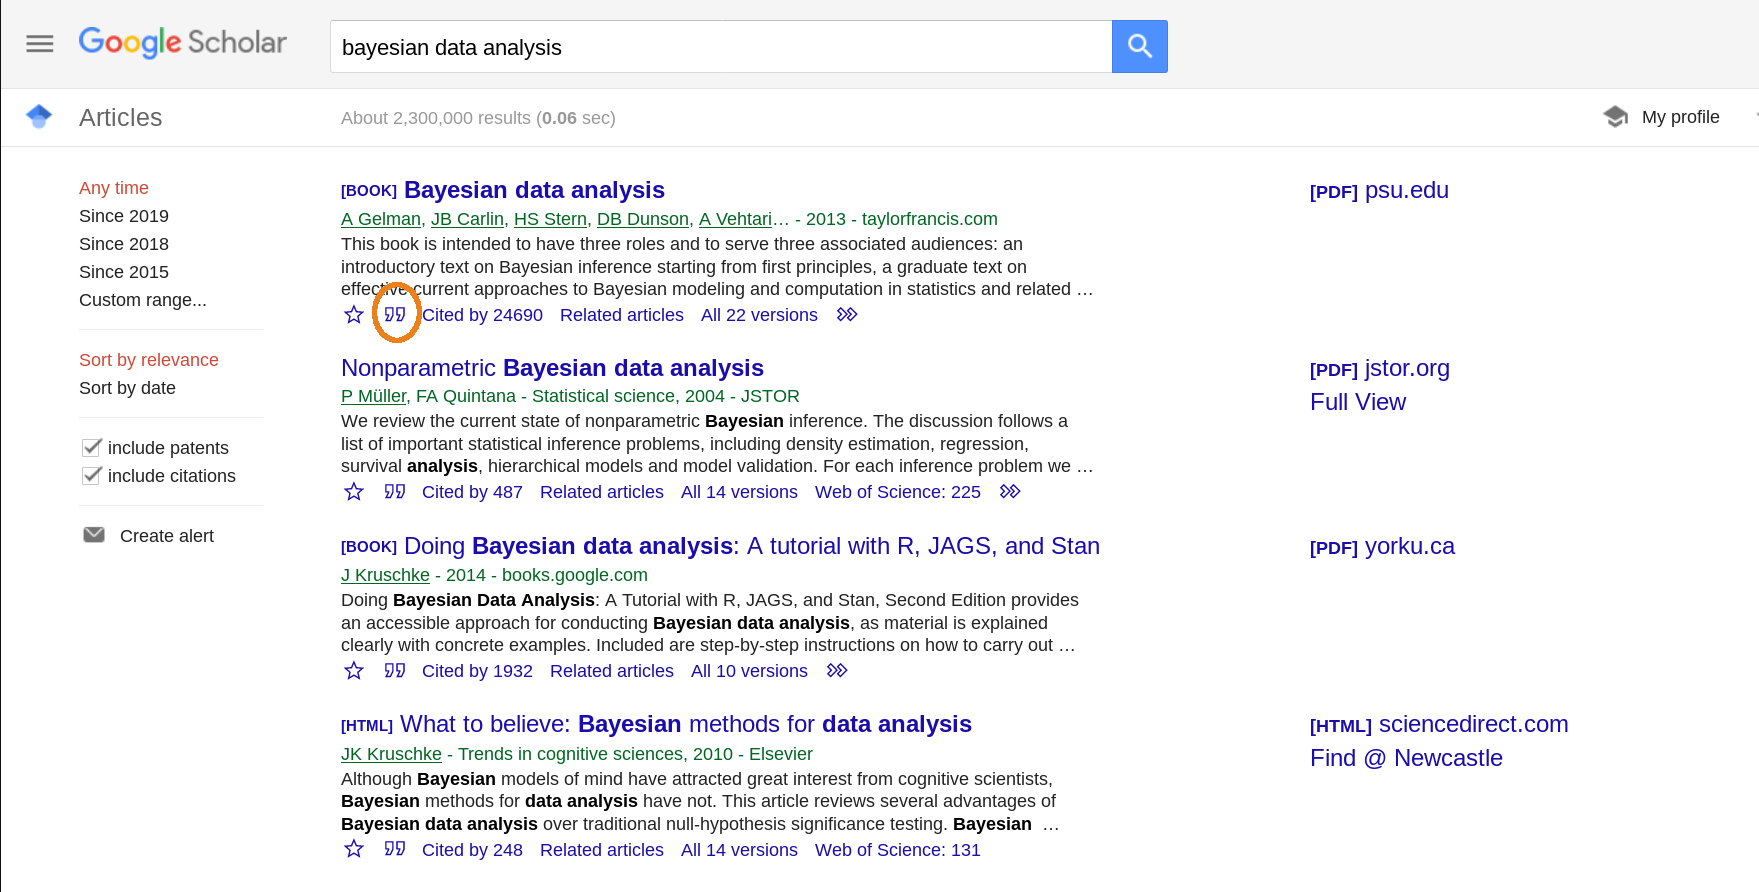
\includegraphics[width=\textwidth]{scholar_bib1.png}
  \end{figure}
\end{frame}

\begin{frame}{Citations from Google Scholar}
Google scholar can be used to export citations easily.
  \begin{figure}
    \centering
    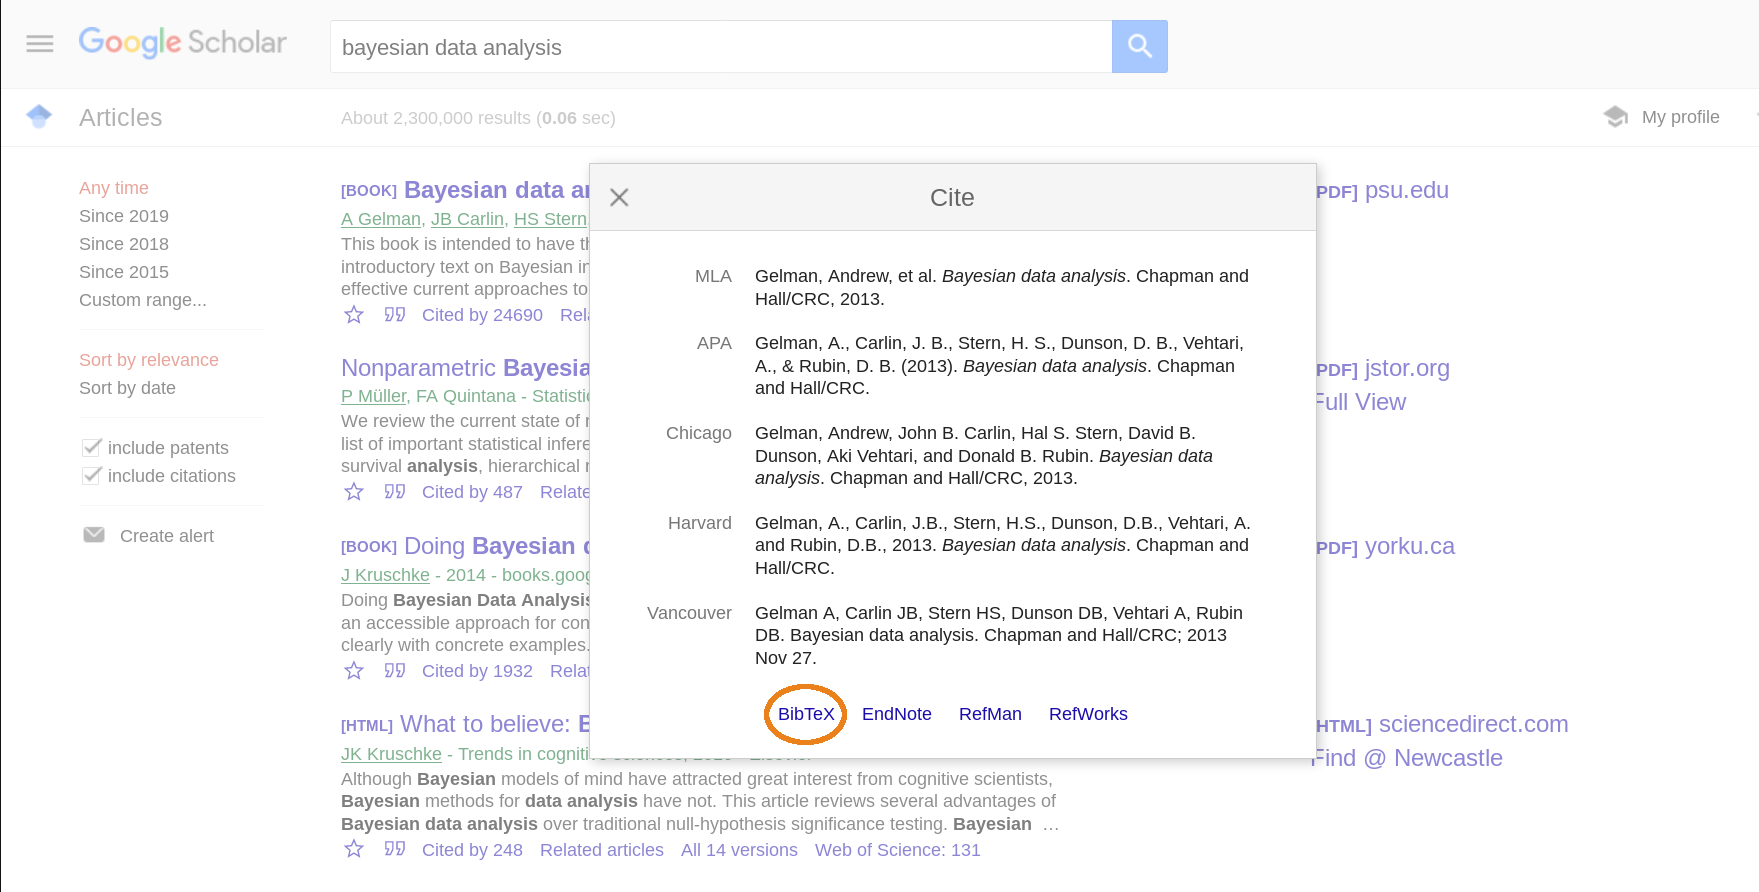
\includegraphics[width=\textwidth]{scholar_bib2.png}
  \end{figure}
\end{frame}

